\documentclass[10pt]{exam}
\usepackage[hon]{template-for-exam}
\usepackage{endnotes,graphicx}
\usepackage{tikz,graphicx,enumitem,multicol,float,my-tikz-clipart,silence}
\graphicspath{{./figures/}}
\WarningFilter{latex}{Label `part}
\WarningFilter{latex}{There were multiply-defined labels}

\footer{}{\thepage}{\sc \myclass}


%\def\answer#1{\footnotetext{#1}}
%\def\myquestion{\item\stepcounter{footnote}}

\def\enoteheading{}
\def\answer#1{\endnotetext{#1}}
\def\theanswers{\theendnotes}
\def\myquestion{\item\stepcounter{endnote}}

\newenvironment{myquestions}{
  \begin{multicols*}{2}\begin{enumerate}
}{
  \end{enumerate}\end{multicols*}
}
\makeatletter
\patchcmd{\enit@setresumekeys}{\def}{\gdef}{}{}
\patchcmd{\enit@setresumekeys}{\def}{\gdef}{}{}
\makeatother

\newcommand{\myheading}[1]{\uplevel{\section*{#1}}
}
\newcommand{\mysubheading}[1]{\uplevel{\subsection*{#1}}
}



\def\mytitle{Chapter 7 Homework (Work \& Energy)}
\title{\mytitle}
\author{Rohrbach}
\date{\today}

\def\mymaketitle{
  \begin{flushleft}
    {\LARGE \textbf \mytitle \par}
  \end{flushleft}
}

\newcommand{\bs}[2]{\textbf{#1} (\sc #2 Points)}


\begin{document}
\maketitle


%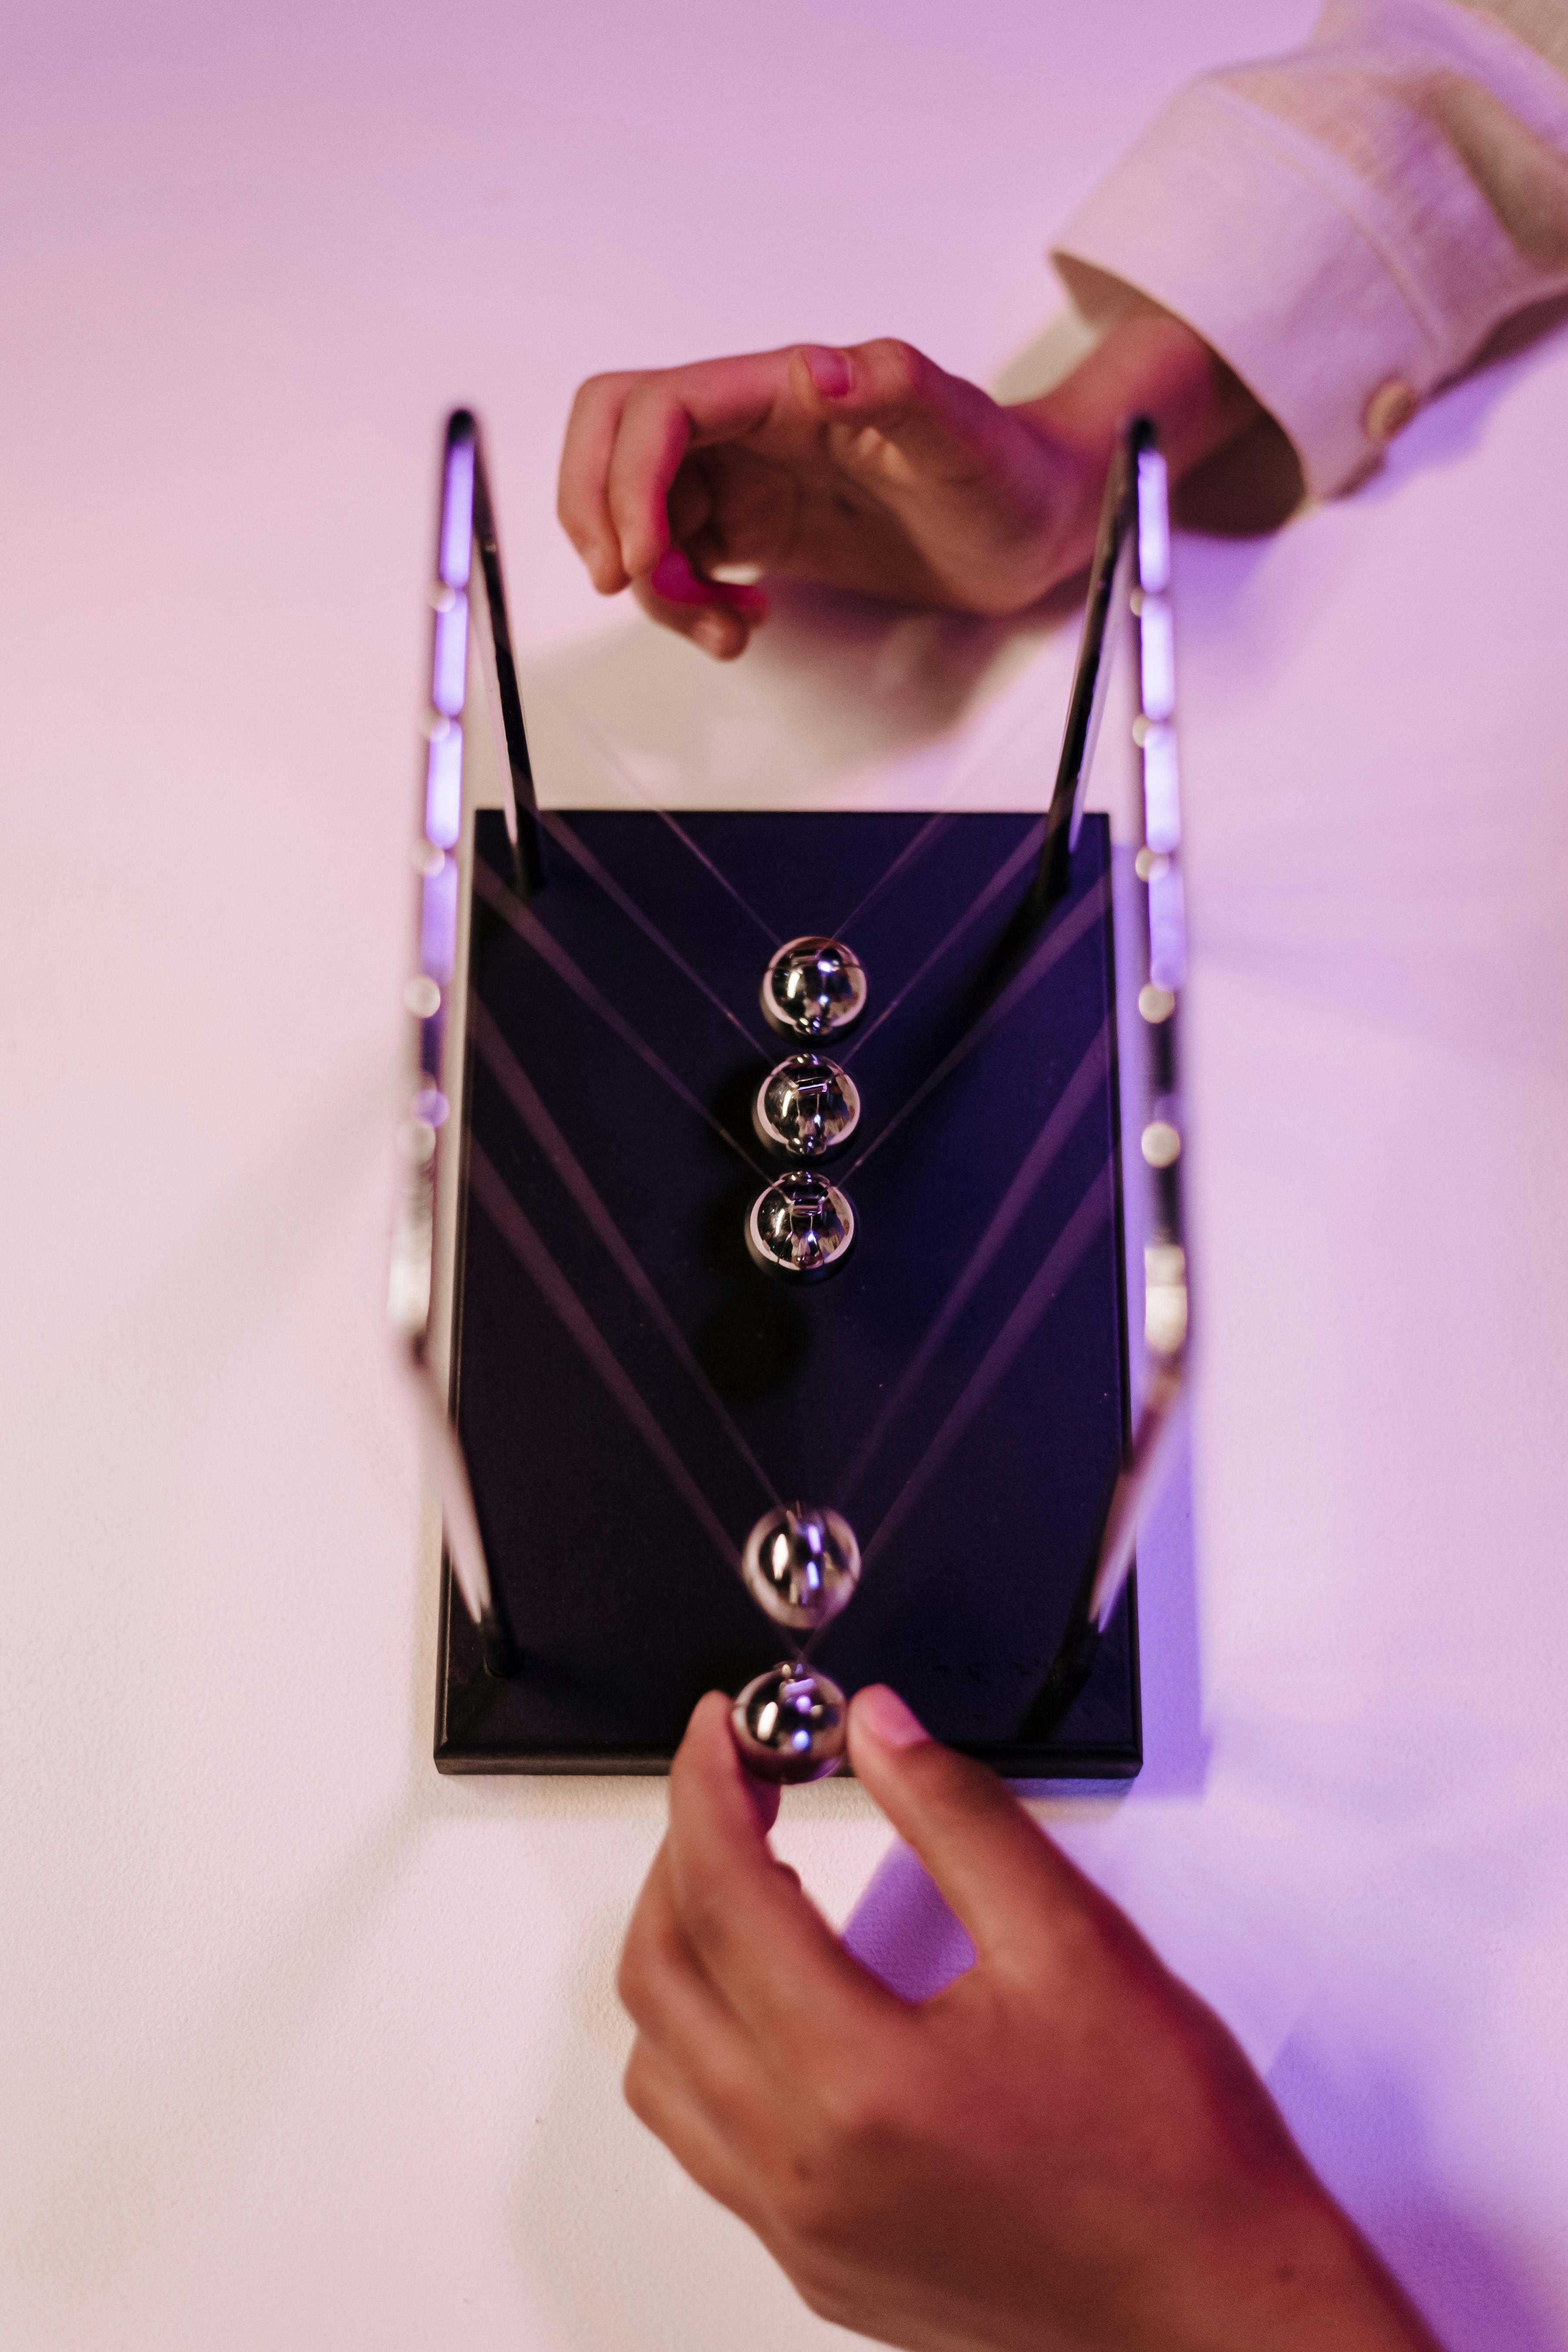
\includegraphics[height=4.5cm]{ncradle.jpg} \hspace{10em}

\section*{All Homework (collected on Wed, Dec 10 / Thu, Dec 11)}


%%%%%%%%%%%

\subsection*{Reading}

Please read the following on your own in the OpenStax textbook by the dates given.  It will give good context for class discussion.  Check off when you have completed them.

\vspace{1em}

\begin{checkboxes}
  \choice 7.1 Work: The Scientific Definition \dotfill Mon, Dec 1
  \choice 7.2 Kinetic Energy \& the Work-Energy Theorem \dotfill Mon, Dec 1
  \choice 7.3 Gravitational Potential Energy \dotfill Mon, Dec 1
  \choice 7.4 Conservative Forces \& Potential Energy \dotfill Mon, Dec 1
  \choice 7.5 Nonconservative Forces \dotfill Wed, Dec 3 / Thu, Dec 4
  \choice 7.6 Conservation of Energy \dotfill Wed, Dec 3 / Thu, Dec 4
  \choice 7.7 Power \dotfill Mon, Dec 8
\end{checkboxes}


\subsection*{Problems and Conceptual Question}


Get stamps from your instructor as you complete each of the following problems.  The conceptual questions (CQ) require at least one sentence of explanation.

\vspace{1em}

\noindent
{\sc Stamps will not be given if work is not shown on a separate sheet of paper}

\vspace{1em}


\begin{tabular}{|*{3}{p{4.8cm}|}}
  \hline
  %
  \bs{Work}{3}               
          & \bs{Kinetic Energy}{2} 
          & \bs{Potential Energy}{3} \\
  Problems \#\ref{work-i}-\ref{work-f}
          & Problems \#\ref{ke-i}-\ref{ke-f} 
          & Problems \#\ref{pe-i}-\ref{pe-f}\\
  Conceptual \#\ref{work-cq-i}-\ref{work-cq-f}
          & Conceptual \#\ref{ke-cq-i}-\ref{ke-cq-f}
          & Conceptual \#\ref{pe-cq-i}-\ref{pe-cq-f} \\
          & & \\[3em]\hline
  %%
  %%
  \bs{Cons. of Energy}{7}               
      & \bs{Power}{5} \\
  Problems \#\ref{cons-i}-\ref{cons-f} 
      & Problems \#\ref{pow-i}-\ref{pow-f}  \\
  Conceptual \#\ref{cons-cq-i}-\ref{cons-cq-f} 
      & Conceptual \#\ref{pow-cq}  \\
      \textbf{HW Quiz {\small W-Th, Dec 10-11}} & \\[3em]\cline{1-2}
  %
\end{tabular}

\subsection*{Bonus Problems}

\hfill

\begin{tabular}{|*{3}{p{3.3cm}|}}
  \hline
  %
  \#\ref{b1}  &  \#\ref{b2}  &  \#\ref{b3} \\[1.5cm]
  %
  \hline
\end{tabular}


\section*{Equations}


\begin{align*}
  W    &\equiv F_\parallel d = Fd\cos\theta &
  KE   &\equiv \frac{1}{2} mv^2 &
  PE_g &= mgh &
  PE_e &= \frac{1}{2} kx^2
\end{align*}


\begin{align*}
  W &= \Delta KE &
  \Sigma E_0 + W_{NC} &= \Sigma E &
  P &\equiv \frac{W}{t}
\end{align*}


\section*{Selected Answers}

\renewcommand{\enotesize}{\normalsize}
\renewcommand{\enoteformat}{%
  \leftskip=1.8em
  \makebox[0pt][r]{\theenmark. }%
}

\hfill
\theanswers

%%%%%%%%%%%%%
%%%%%%%%%%%%%


\pagebreak 



\noindent
Questions and figures are from OpenStax \emph{College Physics}, 2nd ed, (Chapter 7) or Giancolli \emph{Physics: Principles with Applications}, 7th ed, (Chapter 6) unless otherwise noted.
 unless otherwise noted.



\begin{myquestions}

\myheading{Work}
\mysubheading{Problems}

\myquestion (P1) \label{work-i}
How much work does a supermarket checkout attendant do on a can of soup he pushes 0.600 m horizontally with a force of 5.00 N? \answer{3.00~J}

\myquestion (P2) 
A 75.0-kg person climbs stairs, gaining 2.50 meters in height. Find the work done to accomplish this task. (Neglect friction in your calculations.) \answer{1838~J}

\myquestion (P6) \label{work-f}
How much work is done by the boy pulling his sister 30.0 m in a wagon as shown in Figure~\ref{7.33}? Assume no friction acts on the wagon. \answer{1300~J}

  \begin{figure}[H]
    \centering
    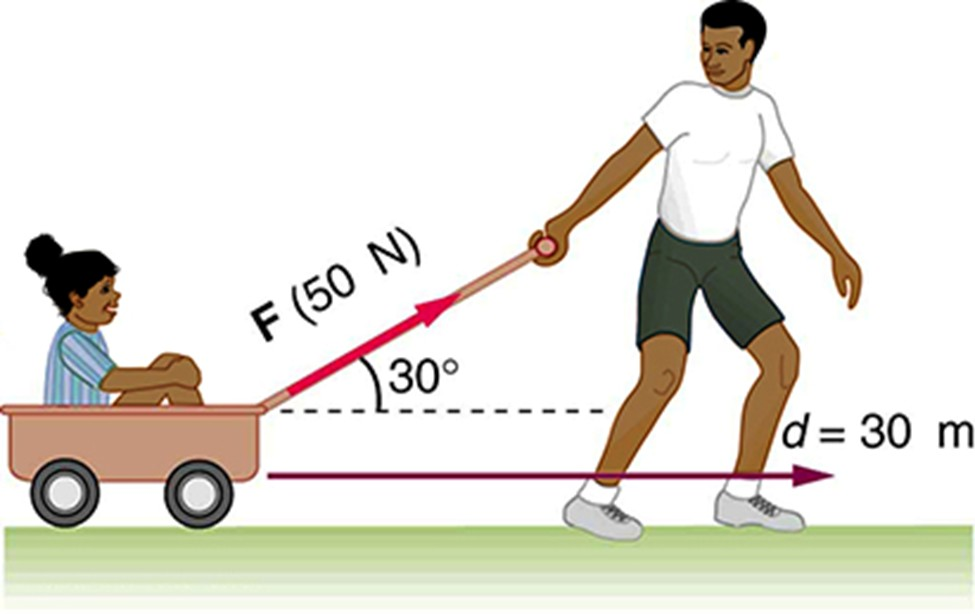
\includegraphics[width=4.5cm]{7-33.jpg}
    \caption{(OpenStax Figure 7.33) The boy does work on the system of the wagon and the child when he pulls them as shown. }
    \label{7.33}
  \end{figure}

  
% \myquestion (P18) 
% Suppose a 350-g kookaburra (a large kingfisher bird) picks up a 75-g snake and raises it 2.5 m from the ground to a branch. (a) How much work did the bird do on the snake? (b) How much work did it do to raise its own center of mass to the branch?

\myquestion \textbf{Bonus} (Giancolli P7) \label{b1}
In a certain library, the first shelf is 15.0~cm off the ground, and the remaining four shelves are each spaced 38.0~cm above the previous one.  If the average book has a meass of 1.40~kg with a height of 22.0~cm, and an average shelf holds 28 books (standing vertically), how much work is required to fill all the shelves, assuming the books are all laying flat on the floor to start?

\uplevel{\subsection*{Conceptual Questions}}

\myquestion (Giancolli CQ2) \label{work-cq-i}
Can a centripetal force ever do work on an object? Explain.

\myquestion (Giancolli CQ4)
Can the normal force on an object ever do work? Explain.


\myquestion (Giancolli MC1) \label{work-cq-f}
You push very hard on a heavy desk, trying to move it. You do work on the desk in which of the following situations? \answer{B}
\begin{parts}
  \part whether or not it moves, as long as you are exerting a force.
  \part only if it starts moving.
  \part only if it doesn't move.
  \part never—it does work on you.
  \part None of the above.
\end{parts}

\myheading{Kinetic Energy}
\mysubheading{Problems}

% \myquestion (P9)
% Compare the kinetic energy of a 20,000-kg truck moving at 110 km/h with that of an 80.0-kg astronaut in orbit moving at 27,500 km/h.

\myquestion (Original Question) \label{ke-i}
  What is the speed of a 1500-kg airplane with 7,350,000 J of Kinetic Energy? \answer{99.0 m/s}

\myquestion (P10) \label{ke-f}
(a) How fast must a 3000-kg elephant move to have the same kinetic energy as a 65.0-kg sprinter running at 10.0 m/s? (b) Discuss how the larger energies needed for the movement of larger animals would relate to metabolic rates. \answer{$KE=3250$~J; $v=1.47$~m/s}

% \myquestion (Ch 6, P15 from Giancolli \textit{Physics: Principles with Applications}, 7th ed.)
% At room temperature, an oxygen molecule, with mass of \SI{5.31e-26}{kg}, typically has a kinetic energy of about \SI{6.21e-21}{J}. How fast is it moving?

\mysubheading{Conceptual Questions}


\myquestion (Giancolli P16) \label{ke-cq-i}
(a) If the kinetic energy of a particle is tripled, by what factor has its speed increased?
(b) If the speed of a particle is halved, by what factor does its kinetic energy change? \answer{(a) $\sqrt{3}$; (b) $1/4$}

\vs \pagebreak
\myquestion (Original Question) \label{ke-cq-f}
Two cars are traveling down the highway. Car \#1 has three times speed as Car \#2, but Car \#2 has four times the mass of Car \#1. Which car has the larger kinetic energy, and by how much? \answer{$KE_1=\frac{9}{4}KE_2$}

    \begin{figure}[H]
      \centering
      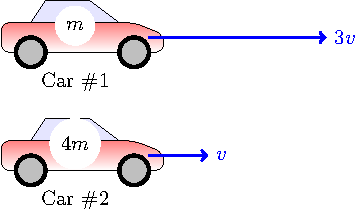
\includegraphics[width=5cm]{cars.pdf}
      \caption{(Original Diagram) Car \#1 has three times speed as Car \#2, but Car \#2 has four times the mass of Car \#1.}
      \label{cars}
    \end{figure}

\myheading{Potential Energy}
\mysubheading{Problems}

\myquestion (P16) \label{pe-i}
A hydroelectric power facility (see Figure~\ref{7.35}) converts the gravitational potential energy of water behind a dam to electric energy. (a) What is the gravitational potential energy relative to the generators of a lake of volume \SI{50}{km^3} (mass = \SI{5.00e13}{kg}), given that the lake has an average height of 40.0~m above the generators? (b) Compare this with the energy stored in a 9-megaton fusion bomb (\SI{3.8e16}{J}). \answer{\SI{1.96e16}{J}; about half the energy of a fusion bomb}
   
\begin{figure}[H]
  \centering
  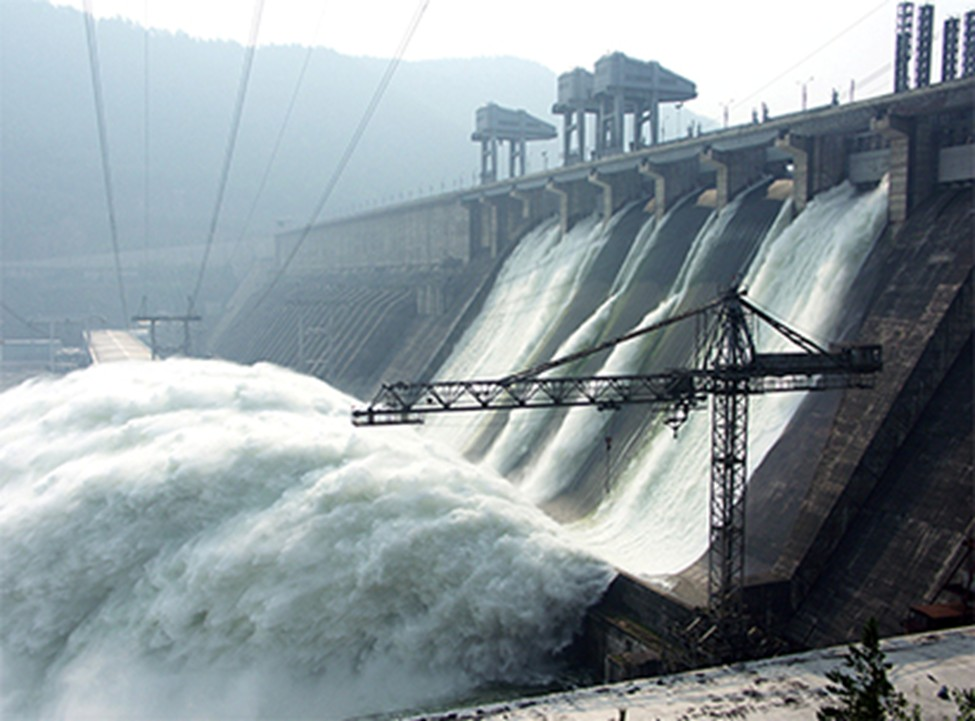
\includegraphics[width=4cm]{7-35.jpg}
  \caption{(OpenStax Figure 7.35) Hydroelectric facility (credit: Denis Belevich, Wikimedia Commons)}
  \label{7.35}
\end{figure}


\myquestion (Giancolli P27)
A spring has a spring constant $k$ of 88.0~N/m. How much must this spring be compressed to store 45.0~J of potential energy? \answer{1.01~m}

% \myquestion (Giancolli P28)
% If it requires 6.0 J of work to stretch a particular spring by 2.0 cm from its equilibrium length, how much more work will be required to stretch it an additional 4.0 cm?


\myquestion (Original Question) \label{pe-f}
Calculate the \emph{total mechanical energy} of a 0.56-kg football thrown.  At the top of its flight, it has a speed of 22~m/s and it is 6.8~m off the ground. \answer{172.8 J}



\mysubheading{Conceptual Questions}

\myquestion (CQ9) \label{pe-cq-i}
What is a conservative force?

\myquestion (CQ8) 
Does the work you do on a book when you lift it onto a shelf depend on the path taken? On the time taken? On the height of the shelf? On the mass of the book?

\myquestion (CQ12) \label{pe-cq-f}
What is the relationship of potential energy to conservative force?



\myheading{Conservation of Energy}
\mysubheading{Problems}


% \myquestion (Giancolli P33)
% A sled is initially given a shove up a frictionless 23.0$^\circ$ incline. It reaches a maximum vertical height 1.22~m higher than where it started at the bottom. What was its initial speed?

% \myquestion (P27, modified) 
% Using energy considerations and assuming negligible air resistance, what is the final speed of a rock thrown from a bridge 20.0~m above water with an initial speed of 15.0 m/s when it hits the water?  Note that this answer is independent of the direction that the rock is thrown.  \answer{24.8 m/s}

\myquestion (Original Question) \label{cons-i}
A 1750-kg car is initially at rest on a flat surface. The driver accelerates the car, covering a distance of 87~meters. The net force acting on the car averages out to 4800~Newtons.  What is the final velocity of the car? \answer{21.8 m/s}

\myquestion (P22) 
A \SI{5.00e5}{kg} subway train is brought to a stop from a speed of 0.500~m/s in 0.400~ m by a large spring bumper at the end of its track. What is the force constant $k$ of the spring? \answer{\SI{7.81e5}{N/m}}


\myquestion (Giancolli P38)
A 62-kg trampoline artist jumps upward from the top of a platform with a vertical speed of 4.5 m/s. (a) How fast is he going as he lands on the trampoline, 2.0 m below (Figure~\ref{G6-40})?  (b) If the trampoline behaves like a spring of spring constant \SI{5.8e4}{N/m}, how far down does he depress it? \answer{(a) 7.7 m/s; (b) 25 cm}

\begin{figure}[H]
  \centering
  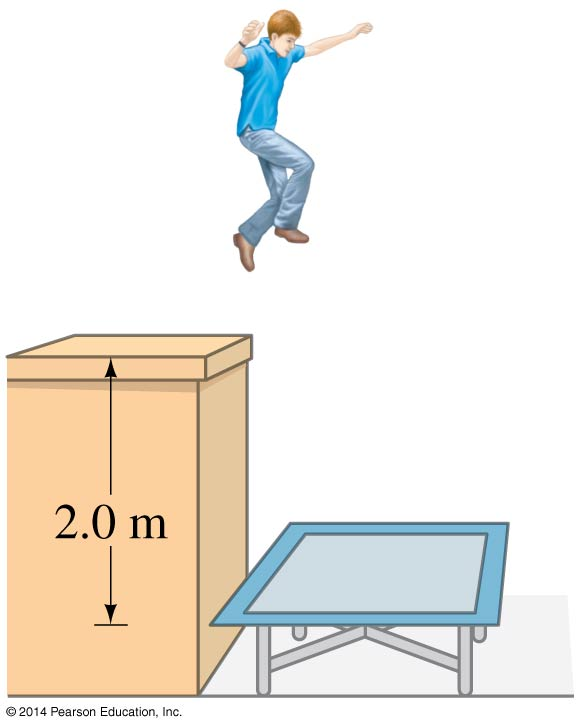
\includegraphics[width=3cm]{06_40_Figure.jpg}
  \caption{Giancolli Figure 6-40}
  \label{G6-40}
\end{figure}



% \myquestion (Original Question)
%   A 2-kg block is kicked up a ramp with an initial speed of 5~m/s, as shown in Figure~\ref{block}.  (a) Assuming no friction, how high up the ramp would the block reach? (b) Instead, the block only makes it up 1.1~meters.  How much work was done by friction? \answer{(a) \SI{1.28}{\meter}; (b) \SI{3.44}{\joule}}

%     \begin{figure}[H]
%       \centering
%       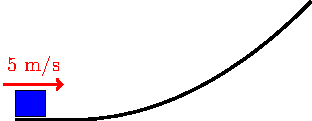
\includegraphics{block.pdf}
%       \caption{(Original Diagram) A block kicked up a ramp with an initial speed of 5~m/s}
%       \label{block}
%     \end{figure}

% \myquestion (Original Question)
%   A roller coaster of mass 1000~kg starts from rest at the top of a 50 m hill, as shown in Figure~\ref{coaster}.  The tracks are frictionless. (a) How fast is it going when it gets to the ground.  (b) How fast is it going when it gets to the top of the next hill, which is 35~m tall?  (c) Now, let’s add friction to this problem. With friction, the roller coaster does not make it to the top of the second hill; instead, it only reaches a height of 32 m before stopping. How much work is done by friction? \answer{(a) 31.3 m/s; (b) 17.1 m/s; (c)$-176,400$~J}

%     \begin{figure}[H]
%       \centering
%       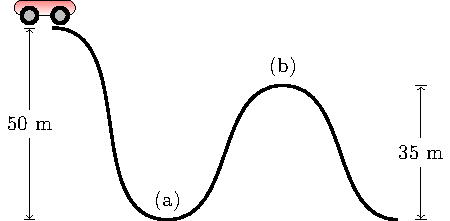
\includegraphics[height=3.3cm]{coaster.pdf}
%       \caption{(Original Diagram) A roller coaster.}
%       \label{coaster}
%     \end{figure}


\myquestion (P24, modified) \label{cons-f}
A 60.0-kg skier with an initial speed of 12.0 m/s coasts up a 2.50-m-high rise as shown in Figure~\ref{7.37}. Find her final speed at the top, given that friction does 168~J of nonconservative work on her. \answer{9.46~m/s}

    \begin{figure}[H]
      \centering
      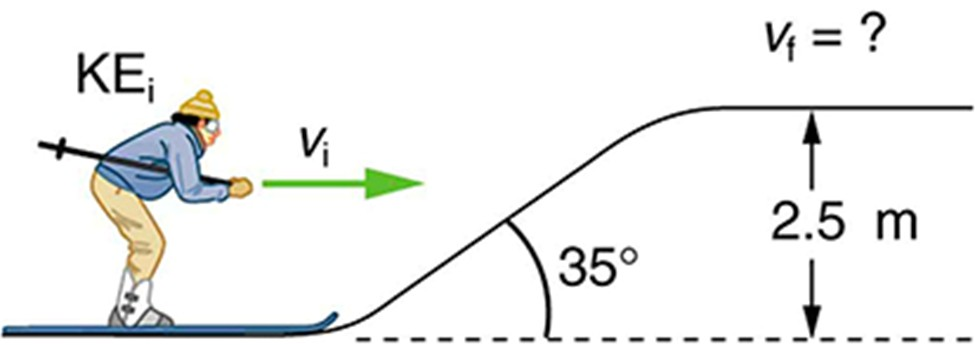
\includegraphics[width=7cm]{7-37.jpg}
      \caption{(OpenStax Fig 7.37) The skier's initial kinetic energy is partially used in coasting to the top of a rise.}
      \label{7.37}
    \end{figure}

\myquestion \textbf{Bonus} (Giancolli P41) \label{b2}
Chris jumps off a bridge witha  bungee cord (a heavy stretchable cord) tied around his ankle, as shown in Figure~\ref{G6-42}.  He fall for 15~m before the bugee cord begins to stretch.  Chris's mass is 75~kg and we assume the cord obeys Hooke's law with $k=55$~N/m.  If we neglect air resistance, estimate the distance $d$ below the bridge Chris's foot will be before coming to a stop.  Ignore the mass of the cord (not realistic, however) and treat Chris as a particle.

    \begin{figure}[H]
      \centering
      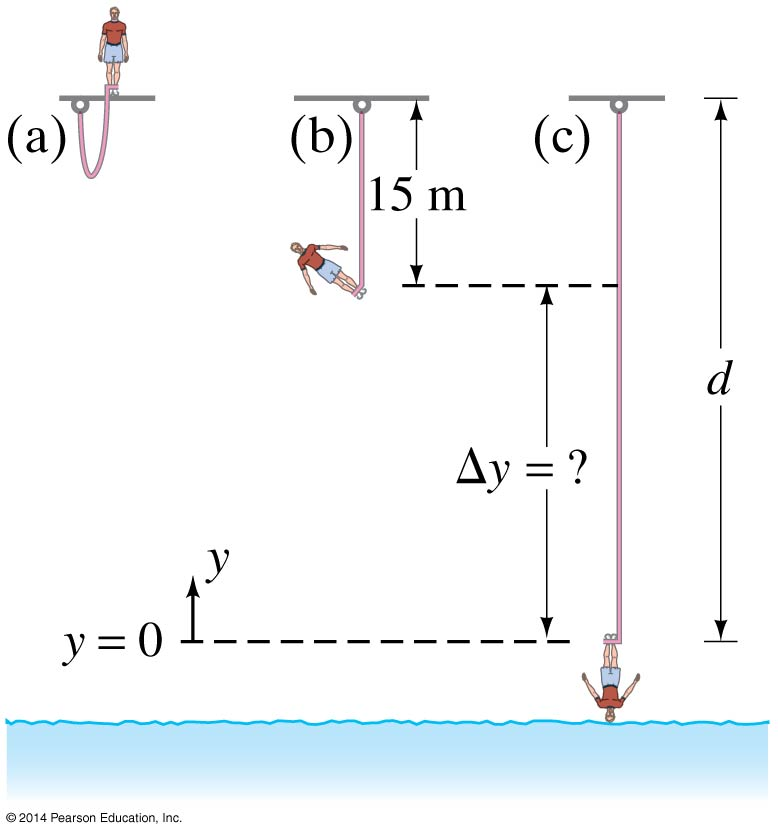
\includegraphics[height=7cm]{06_42_Figure.jpg}
      \caption{(Giancolli Fig 6-42) (a) Bungee jumper about to jump.  (b) Bungee cord at its unstretched length.  (c) Maximum stretch of cord}
      \label{G6-42}
    \end{figure}

\mysubheading{Conceptual Questions}

% \myquestion (CQ13) Consider the following scenario. A car for which friction is not negligible accelerates from rest down a hill, running out of gasoline after a short distance. The driver lets the car coast farther down the hill, then up and over a small crest. He then coasts down that hill into a gas station, where he brakes to a stop and fills the tank with gasoline. Identify the forms of energy the car has, and how they are changed and transferred in this series of events. (See Figure~\ref{7.31}.)

%     \begin{figure}[H]
%       \centering
%       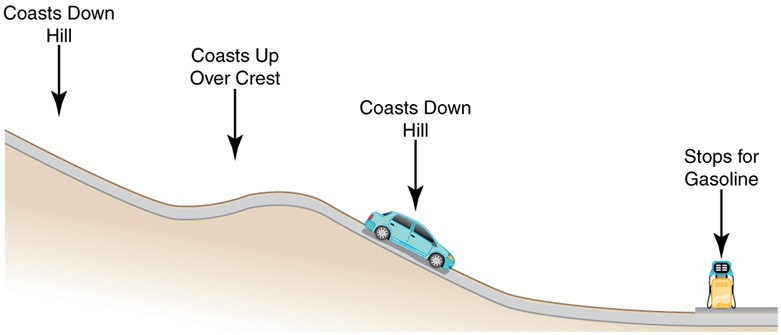
\includegraphics[width=8cm]{7-31.jpg}
%       \caption{(OpenStax Fig 7.31) A car experiencing non-negligible friction coasts down a hill, over a small crest, then downhill again, and comes to a stop at a gas station.}
%       \label{7.31}
%     \end{figure}

\myquestion (Giancolli CQ13) \label{cons-cq-i}
What happens to the gravitational potential energy when water at the top of a waterfall falls to the pool below?


\myquestion (Giancolli MC9, modified) 
Two balls are thrown off a building with the same speed, one straight up and one at a 45$^\circ$ angle. Which ball will have the greater final speed just before it hits the ground? \answer{same speed}

\myquestion (Giancolli MC10, modified) \label{cons-cq-f}
A skier starts from rest at the top of each of the hills shown in Figure~\ref{G6-34}.  There is no friction.  Rank the final velocities of the skier at the bottom of each hill \answer{$v_a=v_b<v_c=v_d$}

\begin{figure}[H]
  \centering
  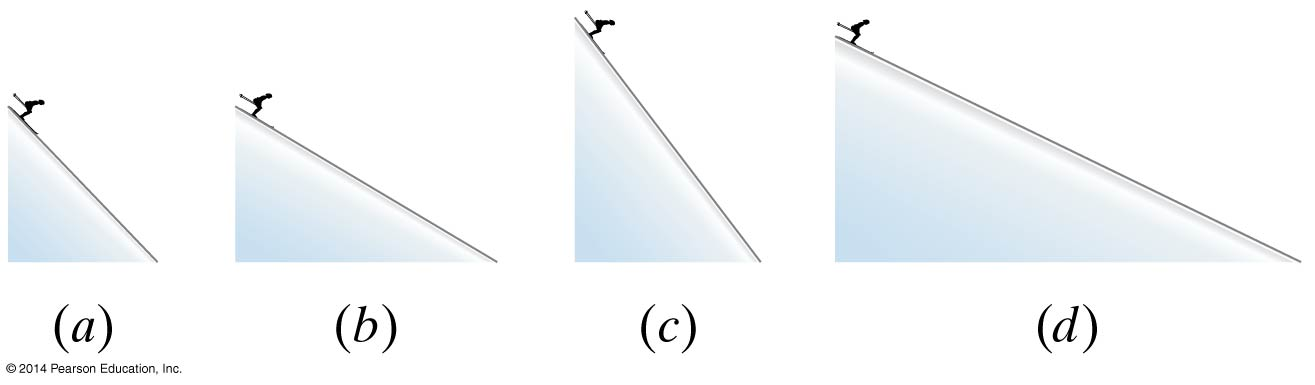
\includegraphics[width=8cm]{06_34_Figure.jpg}
  \caption{Giancolli Figure 6-34}
  \label{G6-34}
\end{figure}



\myheading{Power}
\mysubheading{Problems}

% \myquestion (P36)
% (a) What is the average useful power output of a person who does \SI{6.0e6}{J}  of useful work in \SI{8.00}{hr}? (b) Working at this rate, how long will it take this person to lift 2000 kg of bricks 1.50 m to a platform? (Work done to lift his body can be omitted because it is not considered useful output here.)

\myquestion (P40) \label{pow-i}
(a) What is the available energy content, in joules, of a battery that operates a 2.00-W electric clock for 18 months? (b) How long can a battery that can supply \SI{8.00e4}{J}  run a pocket calculator that consumes energy at the rate of \SI{1.00e-3}{W}? \answer{(a) \SI{9.46e7}{J}; (b) \SI{2.54}{yr}}


\myquestion (Giancolli P57)
How long will it take a 2750-W motor to lift a 385-kg piano to a sixth-story window 16.0 m above? \answer{21.95 s}

% \myquestion (Giancolli P59)
% An 85-kg football player traveling 5.0 m/s is stopped in 1.0~s by a tackler.(a) What is the original kinetic energy of the player? (b) What average power is required to stop him?


\myquestion (Giancolli P60) \label{pow-f}
If a car generates 18 hp when traveling at a steady 25~m/s, what must be the average force exerted on the car due to friction and air resistance? ($\SI{1}{hp}=\SI{746}{W}$) \answer{508.8 N}

% \myquestion (Giancolli P61)
% An outboard motor for a boat is rated at 35~hp.  If it can move a particular boat at a steady speed of 9.5~m/s, what is the toatl force resisting the motion of the boat? ($\SI{1}{hp}=\SI{746}{W}$) \answer{2,686 N}

\myquestion \textbf{Bonus!} (P61) \label{b3}
A 75.0-kg cross-country skier is climbing a $3.0^\circ$ slope at a constant speed of 2.00~m/s and encounters air resistance of 25.0~N. Find his power output for work done against the gravitational force and air resistance. (b) What average force does he exert backward on the snow to accomplish this? (c) If he continues to exert this force and to experience the same air resistance when he reaches a level area, how long will it take him to reach a velocity of 10.0 m/s? \answer{(a) 127 W; (b) 63.5 N; (c) 15.6 s}


\mysubheading{Conceptual Questions}

\myquestion (CQ18) \label{pow-cq}
 Most electrical appliances are rated in watts. Does this rating depend on how long the appliance is on? (When off, it is a zero-watt device.) Explain in terms of the definition of power.



\end{myquestions}

\end{document}